\documentclass[letterpaper,12pt,oneside]{article}\usepackage[]{graphicx}\usepackage[]{color}
%% maxwidth is the original width if it is less than linewidth
%% otherwise use linewidth (to make sure the graphics do not exceed the margin)
\makeatletter
\def\maxwidth{ %
  \ifdim\Gin@nat@width>\linewidth
    \linewidth
  \else
    \Gin@nat@width
  \fi
}
\makeatother

\definecolor{fgcolor}{rgb}{0.345, 0.345, 0.345}
\newcommand{\hlnum}[1]{\textcolor[rgb]{0.686,0.059,0.569}{#1}}%
\newcommand{\hlstr}[1]{\textcolor[rgb]{0.192,0.494,0.8}{#1}}%
\newcommand{\hlcom}[1]{\textcolor[rgb]{0.678,0.584,0.686}{\textit{#1}}}%
\newcommand{\hlopt}[1]{\textcolor[rgb]{0,0,0}{#1}}%
\newcommand{\hlstd}[1]{\textcolor[rgb]{0.345,0.345,0.345}{#1}}%
\newcommand{\hlkwa}[1]{\textcolor[rgb]{0.161,0.373,0.58}{\textbf{#1}}}%
\newcommand{\hlkwb}[1]{\textcolor[rgb]{0.69,0.353,0.396}{#1}}%
\newcommand{\hlkwc}[1]{\textcolor[rgb]{0.333,0.667,0.333}{#1}}%
\newcommand{\hlkwd}[1]{\textcolor[rgb]{0.737,0.353,0.396}{\textbf{#1}}}%

\usepackage{framed}
\makeatletter
\newenvironment{kframe}{%
 \def\at@end@of@kframe{}%
 \ifinner\ifhmode%
  \def\at@end@of@kframe{\end{minipage}}%
  \begin{minipage}{\columnwidth}%
 \fi\fi%
 \def\FrameCommand##1{\hskip\@totalleftmargin \hskip-\fboxsep
 \colorbox{shadecolor}{##1}\hskip-\fboxsep
     % There is no \\@totalrightmargin, so:
     \hskip-\linewidth \hskip-\@totalleftmargin \hskip\columnwidth}%
 \MakeFramed {\advance\hsize-\width
   \@totalleftmargin\z@ \linewidth\hsize
   \@setminipage}}%
 {\par\unskip\endMakeFramed%
 \at@end@of@kframe}
\makeatother

\definecolor{shadecolor}{rgb}{.97, .97, .97}
\definecolor{messagecolor}{rgb}{0, 0, 0}
\definecolor{warningcolor}{rgb}{1, 0, 1}
\definecolor{errorcolor}{rgb}{1, 0, 0}
\newenvironment{knitrout}{}{} % an empty environment to be redefined in TeX

\usepackage{alltt}
\usepackage[paperwidth=8.5in,paperheight=11in,top=1in,bottom=1in,left=1in,right=1in]{geometry}
\usepackage{setspace}
\usepackage[colorlinks=true,allcolors=Blue]{hyperref}
\usepackage[usenames,dvipsnames]{xcolor}
\usepackage{indentfirst}
\usepackage{titlesec}
\usepackage{multirow}
\usepackage{booktabs}
\usepackage{graphicx}
\usepackage{verbatim}
\usepackage{rotating}
\usepackage{tabularx}
\usepackage{outlines}
\usepackage{lineno}
\usepackage{array}
\usepackage{times}
\usepackage{cleveref}
\usepackage{acronym}
\usepackage[position=t]{subfig}
\usepackage{paralist}
\usepackage[noae]{Sweave}
\usepackage{natbib}
\usepackage{array}
\usepackage{pdflscape}
\usepackage{bm}
\usepackage{showlabels}
\bibpunct{(}{)}{,}{a}{}{,}

% page margins and section title formatting
\linespread{1.5}
\setlength{\footskip}{0.5in}
\titleformat*{\section}{\Large\bf\em}
\titleformat*{\subsection}{\singlespace\large\bf}
\titleformat*{\subsubsection}{\singlespace\normalsize\bf\em}
\titlespacing{\section}{0in}{0in}{0in}
\titlespacing{\subsection}{0in}{0in}{0in}
\titlespacing{\subsubsection}{0in}{0in}{0in}

% cleveref options
\crefname{table}{Table}{Tables}
\crefname{figure}{Fig.}{Figs.}
\renewcommand{\figurename}{Fig.}

% aliased citations
\defcitealias{HagyIR}{Hagy, In review}
\defcitealias{USEPA06}{USEPA, 2006}
\defcitealias{USEPA98}{USEPA, 1998}

%acronyms
\acrodef{BB}{Big Bend}
\acrodef{DEM}{Digital Elevation Model}
\acrodef{EPA}{Environmental Protection Agency}
\acrodef{doc}[$Z_c$]{depth of colonization}
\acrodef{GIS}{Geographic Information System}
\acrodef{IWR}{Impaired Waters Rule}
\acrodef{MSL}{mean sea level}
\acrodef{NAVD88}{North American Vertical Datum of 1988}
\acrodef{NOAA}{National Oceanic and Atmospheric Administration}
\acrodef{OTB}{Old Tampa Bay}
\acrodef{UIRL}{Upper Indian River Lagoon}
\acrodef{WCB}{Western Choctawhatchee Bay}

%knitr options


\IfFileExists{upquote.sty}{\usepackage{upquote}}{}
\begin{document}

\raggedbottom
\linenumbers
\raggedright
\urlstyle{same}
\setlength{\parindent}{0.5in}
\renewcommand\refname{References \vspace{12pt}}

\begin{singlespace}
\title{{\bf {\Large Quantifying seagrass light requirements using an algorithm to spatially resolve depth of colonization}}}
\author{
  {\bf {\normalsize Marcus W. Beck$^1$, James D. Hagy III$^2$}}
  \\\\{\textit {\normalsize $^1$ORISE Research Participation Program}}
  \\{\textit {\normalsize USEPA National Health and Environmental Effects Research Laboratory}}
  \\{\textit {\normalsize Gulf Ecology Division, 1 Sabine Island Drive, Gulf Breeze, FL 32561}}
	\\{\textit {\normalsize Phone: 850-934-2480, Fax: 850-934-2401, Email: \href{mailto:beck.marcus@epa.gov}{beck.marcus@epa.gov}}}
  \\\\{\textit {\normalsize $^2$USEPA National Health and Environmental Effects Research Laboratory}}
	\\{\textit {\normalsize Gulf Ecology Division, 1 Sabine Island Drive, Gulf Breeze, FL 32561}}
	\\{\textit {\normalsize Phone: 850-934-2455, Fax: 850-934-2401, Email: \href{mailto:hagy.jim@epa.gov}{hagy.jim@epa.gov}}}
	}
\date{}
\maketitle
\end{singlespace}
\clearpage

\section{Introduction}

Seagrasses are ecologically valuable components of aquatic systems that serve a structural and functional role in shaping aquatic habitat.  These `ecosystem engineers' often govern multiple characteristics of aquatic systems through direct and indirect interactions with additional components \citep{Jones94,Koch01}.  For example, seagrass beds create desirable habitat for juvenile fish and invertebrates by reducing wave action and stabilizing sediment \citep{williams01,Hughes09}.  Seagrasses also respond to changes in water clarity through direct physiological linkages with light availability.  Seagrass communities in highly productive aquatic systems may be light-limited as increased nutrient loading may contribute to reductions in water clarity through increased algal concentration \citep{Duarte95}.  Empirical relationships between nutrient loading, water clarity, light requirements, and the maximum depth of seagrass colonization have been identified \citep{Duarte91,Kenworthy96,Choice14} and are often used to characterize light regimes sufficient to maintain habitat through increased seagrass coverage \citep{Steward05}.  Seagrass depth limits have also been used to establish quantititative criteria for nutrient load targets for the maintenance of water quality \citep{Janicki96}.  Seagrasses are integrative of system-wide conditions over time in relation to changes in nutrient regimes \citep{Duarte95} and are often preferred biological endpoints to describe ecosytem response to perturbations relative to more variable taxa (e.g., phytoplankton).  Quantifying the relationship of seagrasses with water clarity is a viable means of understanding ecological characteristics of aquatic systems with potential insights into resilience and stability of system response to disturbance \citep{Greve05}.    

A variety of techniques have been developed for estimating seagrass depth limits as a basis for understanding water quality dynamics and developing a more robust description of aquatic habitat.  Such efforts have been useful for site-specific approaches where the analysis needs are driven by a particular management or research question \citep[e.g.,][]{Iverson86,Hale04}. However, a lack of standardization among methods has prevented broad-scale comparisons between regions and has even contributed to discrepancies between measures of depth limits based on the chosen technique.  For example, seagrass depth limits based on in situ techniques can vary with the sampling device \citep{Spears09}.  Seagrass depth limits can also be estimated from geospatial data that describe aerial coverage and bathymetric depth distribution.  Despite the availability of such data, flexible techniques for estimating seagrass depth of colonization have not been extensively developed nor have standardized techniques been implemented across broad areas.  Site-specific approaches typically involve the quantification of depth limits within a predefined management unit as a relevant spatial context. For example, \cite{Steward05} describe use of a segmentation scheme for the Indian River Lagoon on the Atlantic coast of Florida to assign seagrass depth limits to 19 distinct geospatial units.  Although useful within a limited scope, substantial variation in growth patterns and water quality characteristics at different spatial scales may prevent more detailed analyses, thus leading to limited descriptions of aquatic habitat.  Methods for estimating seagrass depth limits should be reproducible for broad-scale comparisons, while also maintaining flexibility of  estimates depending on research or managment objectives. Such techniques have the potential to facilitate comparisons between regions given the spatial coverage and annual availability of many geospatial data sources.  

A useful application comparing depth limit measures and water clarity is the estimation of light requirements to evaluate ecologically relevant characterisics of seagrass communities.  Although growth of submersed aquatic plants is generally most limited by light availability \citep{Barko82,Hall90,Dennison93}, substantial variation for a given level of light may be observed in the maximum depth of growth based on differences in light requirements \citep{Dennison93,Choice14}.  In general, seagrasses with low light requirements are expected to grow deeper than seagrasses with high requirements as related to species or regional differences in community attributes.  Significant variation in light requirements in seagrasses along the Gulf Coast of peninsular Florida were attributed to morphological and physiological differences between species and adaptations to regional light regimes \citep{Choice14}.  Minimum light requirements for seagrasses are on average 11\% of surface irradiance \citep{Duarte91}, although values may range from less than 5\% to greater than 30\% at depth \citep{Dennison93}. High light requirements estimated from maximum depth of colonization and water clarity may suggest seagrass growth is limited by additional factors, such as high biomass of epiphytic algal growth that reduces light availability on the leaf surface \citep{Kemp04}. Spatial heterogeneity in light requirements is, therefore, a useful diagnostic tool for evaluating potential factors that limit seagrass growth. 

A potentially limiting factor for estimating seagrass light requirements is the availability of water clarity data that are evenly distributed through space in time, in addition to accurate measures of depth of colonization.  Secchi observations are routine measurements that can provide consistent measures of water clarity \citepalias{USEPA06}, although the distribution of available data may limit the certainty within which light requirements can be estimated.  Secchi data can be biased by location such that monitoring programs may have unbalanced coverage towards aquatic resources with greater perceived importance relative to those that may have more ecological significance \citep{Wagner08,Lottig14}.  Morever, infrequent field measurements that are limited to discrete time periods are often more descriptive of short-term variability rather than long-term trends in water clarity \citep{Elsdon09}.  Seagrasses growth patterns are integrative of seasonal and inter-annual patterns in water clarity, among other factors, such that estimates of light requirements may be limited if water clarity measurements inadequately describe temporal variation.  Remote sensing products can provide a reasonable estimate of water clarity and could be used to develop a more spatially and temporally coherent description of relevant ecosystem characteristics.  Although algorithms have been developed for coastal waters that relate surface reflectance to \textit{in situ} data \citep{Woodruff99,Chen07}, this information has rarely been used to develop a description of seagrass light requirements at a spatial resolution consistent with most remote sensing products.    

Quantitative and flexible methods for estimating seagrass depth limits and light requirements have the potential to greatly improve descriptions of aquatic habitat, thus enabling potentially novel insights into ecological characteristics of aquatic systems.  This article describes a method for estimating seagrass depth of colonization using geospatial datasets to create a spatially-resolved and flexible measure.  In particular, an empirical algorthm is described that estimates seagrass depth limits from aerial coverage maps and bathymetric data using an \textit{a priori} defined area of influence. These estimates are combined with measures of water clarity to provide a spatial characterization of light requirements to better understand factors that limit seagrass growth.  The specific objectives are to\begin{inparaenum}[1\upshape)]
\item describe the method for estimating seagrass depth limits within a relevant spatial context, 
\item apply the technique to four distinct regions of Florida to illustrate improved clarity of description for seagrass growth patterns, and
\item develop a spatial description of depth limits, water clarity, and light requirements for the case studies.  
\end{inparaenum}
The method is first illustrated using four relatively small areas of larger coastal regions folowed by extension to entire bay systems to characterize spatial variation in light requirements.  Overall, these methods are expected to inform the description of seagrass growth patterns to develop a more ecologically relevant characterization of aquatic habitat.  The method is applied to data from Florida although the technique is easily transferable to other regions with comparable data. 

\section{Methods}

Estimates of seagrass \ac{doc} that are derived from relatively broad spatial aggregations, such as predefined management areas, may not fully describe relevant variation depending on the question of interest. \Cref{fig:buff_ex1} shows variation in seagrass distribution for a management segment (thick polygon) in the Big Bend region of Florida.  The maximum depth colonization, shown as a red countour line, is based on a segment-wide average of all seagrasses within the polygon.  Although such an estimate is not necessarily inaccurate, substantial variation in seagrass growth patterns at smaller spatial scales is not adequately described. In particular, \ac{doc} is greatly over-estimated at the outflow of the Steinhatchee River (northeast portion of the segment) where high concentrations of dissolved organic matter reduce water clarity and naturally limit seagrass growth (personal communication, Nijole Wellendorf, Florida Department of Environmental Protection).  This example suggests that it may be useful to have improved spatial resolution in estimates of \ac{doc}, particularly when site-specific characteristics may require a more detailed description of seagrass growth patterns.  The following is a summary of data sources, methods and rationale for developing a flexible algorithm that improves spatial resolution in seagrass \ac{doc} estimates.  Data and methods described in \citetalias{HagyIR} are used as a foundation for developing the approach.

\subsection{Data sources}

\subsubsection{Study sites}

Four locations in Florida were chosen for the analysis: the Big Bend region (northeast Gulf of Mexico), Choctawhatchee Bay (pandhandle), Tampa Bay (central Gulf Coast), and Indian River Lagoon (east coast) (\cref{tab:seg_summ,fig:seg_all}).  These locations represent different geographic regions in the state, in addition to having available data and observed gradients in water clarity that contribute to heterogeneity in seagrass growth patterns. Coastal regions and estuaries in Florida are partitioned into distinct spatial units based on a segmentation scheme developed by US \ac{EPA} for the development of numeric nutrient criteria.  Site-specific estimates of seagrass depth colonization and light requirements are the primary focus of the analysis, with emphasis on improved clarity of description with changes in spatial context.  As such, estimates that use management segments as relevant spatial units are used as a basis of comparison to evaluate variation in growth patterns at difference scales.  The analysis focuses on Choctawhatchee Bay (central pandhandle), the big bend region (northeast pandhandle), Tampa Bay (west coast), and Indian River Lagoon (east coast) .  One segment within each region is first evaluated to illustrate use of the method and variation at relatively small spatial scales.  The segments included a location near the outflow of the Steinhatchee River for the \ac{BB} region, \ac{OTB}, \ac{UIRL}, and \ac{WCB} \cref{fig:seg_all}).  A second analysis focused on describing seagrass depth limits for the entire area of each bay (Choctawhatchee Bay, Tampa Bay, and the Indian River Lagoon) to develop a spatial description of light requirements.

\subsubsection{Seagrass coverage and bathymetry} \label{sec:data_srcs}

Spatial data describing seagrass aerial coverage combined with co-located bathymetric depth information were used to estimate \ac{doc}.  These geospatial data products are publically available in coastal regions of Florida through the US Geological Survey, Florida Department of Environmental Protection, Florida Fish and Wildlife Conservation Commission, and watershed management districts.  Seagrass coverage maps were obtained for recent years in each of the study sites described above (\cref{tab:seg_summ}).  Coverage maps were produced using photo-interpretations of aerial images to categorize seagrass as absent, discontinuous (patchy), or continuous.  For this analysis, we considered seagrass as only present (continuous and patchy) or absent since differences between continuous and patchy coverage were often inconsistent between data sources. 

Bathymetric depth layers for each location were obtained from the National Oceanic and Atmospheric Administration's (\acsu{NOAA}) National Geophysical Data Center (\url{http://www.ngdc.noaa.gov/}) as either \acp{DEM} or raw sounding data from hydroacoustic surveys.  Tampa Bay data provided by the Tampa Bay National Estuary Program are described in \citet{Tyler07}. Bathymetric data for the Indian River Lagoon were obtained from the St. John's Water Management District \citep{CPE97}.  \ac{NOAA} products were referenced to mean lower low water, whereas Tampa Bay data were referenced to the \ac{NAVD88} and the Indian River Lagoon data were referenced to mean sea level.  Depth layers were combined with seagrass coverage layers using standard union techniques for raster and vector layers in ArcMap 10.1 \citep{ESRI12}.  To reduce computation time, depth layers were first masked using a 1 km buffer of the seagrass coverage layer.  Raster bathymetric layers were converted to vector point layers to combine with seagrass coverage maps, described below.  All spatial data were referenced to the North American Datum of 1983 as geographic coordinates.  Depth values in each seagrass layer were further adjusted from the relevant vertical reference datum to local \ac{MSL} using the \ac{NOAA} VDatum tool (\url{http://vdatum.noaa.gov/}).

\subsubsection{Water clarity and light attenuation}

Seagrass light requirements can be estimated by evaluating spatial relationships between depth of colonization and water clarity.  These relationships were explored using \ac{doc} and water clarity estimates for the entire areas of Choctawhatchee Bay, Tampa Bay, and the Indian River Lagoon. Limited data describing water clarity in the Big Bend region prohibited analysis in this location.  Satellite images were used to create a gridded 1 km$^2$ map of light attenuation as either estimated water clarity (m) or light extinction ($K_d$, m$^{-1}$) based on a previously-developed algorithm for Tampa Bay \citep{Chen07}.  Daily MODIS (Aqua level-2) data for the preceding five years from the seagrass coverage layer for each bay were downloaded from the NASA website (\url{http://oceancolor.gsfc.nasa.gov/}). These images were reprocessed using the SeaWiFS Data Analysis System software (SeaDAS, Version 7.0). The clarity algorithm proposed by \citet{Chen07} was used to derive monthly mean, then annual mean light attenuation coefficients for Tampa Bay.  Satellite-estimated water clarity was derived from the light attenuation estimates for Tampa Bay using a conversion equation that was previously validated using in situ data.  A single layer for further analysis was created as the average of all five years.

Light attenuation data for Choctawhatchee Bay were similarly obtained using the clarity algorithm developed for Tampa Bay.  Satellite estimates were retained as light extinction coefficients based on the availability of in situ data obtained from vertical profiles of photosynthetically active radiation.  Light extinction estimates for 2010 were obtained at ten locations in Choctawhatchee Bay at monthly intervals that were used to correct the satellite $K_d$ values.  Monthly field estimates were averaged and compared to the annual mean estimates from the 2010 satellite data.  An empirical correction equation was developed based on the difference between the cumulative distribution of the in situ $K_d$ estimates and the satellite estimates at the same locations.  The 2010 correction was applied to the all five years of annual mean satellite data prior to averaging all data to create a single layer for further analysis. 

Satellite estimates of water clarity were unobtainable in the Indian River Lagoon because of significant light scattering from bottom reflectance and limited resolution for extended narrow segments along the north-south axis.  Secchi data (meters, $Z_{secchi}$) were obtained from update 40 of the \ac{IWR} database for all of the Indian River Lagoon. Secchi data within the previous ten years of the seagrass coverage data were evaluated to capture water quality trends (i.e., 1999--2009).  More than five years of clarity data was used for Indian River Lagoon due to uneven temporal coverage relative to the satellite-based estimates described above.  Stations with less than five observations and observations that were flagged indicating that the value was lower than the maximum depth of the observation point were removed.  Secchi data were also compared with bathymetric data to verify unflagged values were not missed by initial screening. 

\subsection{Estimation of seagrass depth of colonization} \label{sec:est_method}

The approach to estimating seagrass \acl{doc} uses combined seagrass coverage maps and bathymetric depth data described above.  The combined layer used for analysis was a point shapefile with attributes describing location (latitude, longitude, segment), depth (m), and seagrass (present, absent).  Seagrass \ac{doc} values are estimated from these data by quantifying the proportion of points with seagrass at each observed depth.  Three unique measures describing seagrass depth limits obtained from these data are minimum ($Z_{c,\,min}$), median ($Z_{c,\,med}$), and maximum ($Z_{c,\,max}$) \acl{doc}.  Operationally, these terms describe characteristics of the seagrass coverage map with quantifiable significance. $Z_{c,\,max}$ is defined as the deepest depth at which a significant coverage of mappable seagrasses occured independent of outliers, whereas  $Z_{c,\,med}$ is the median depth occurring at the deep water edge. $Z_{c,\,min}$ is the depth at which seagrass coverage begins to decline with increasing depth and may not be statistically distinguishable from zero depth, particularly in turbid waters. Specific methods for estimating each \ac{doc} value using spatially-resolved information are described below. 

The spatially-resolved approach for estimating \ac{doc} begins by choosing an explicit location in cartesian coordinates within the general boundaries of the available data.  Seagrass depth data (i.e., merged bathymetric and seagrass coverage data) that are located within a set radius from the chosen location are selected for estimating seagrass \ac{doc} values (\cref{fig:buff_ex}). The estimate for each location is quantified from a plot of the proportion of sampled points that contain seagrass at decreasing 0.1 meter depth bins from the surface to the maximum observed depth in the sample (\cref{fig:est_ex1}).  Although the chosen radius for selecting depth points is problem-specific, the minimum radius should be chosen to sample a sufficient number of points for estimating \ac{doc}.  In general, an appropriate radius will produce a plot that indicates a decrease in the proportion of points that are occupied by seagrass with increasing depth. If more than one location is used to estimate \ac{doc}, appropriate radii for each point would have minimal overlap with the seagrass depth data sampled by neighboring points.     

A curve is fit to the sampled depth points using non-linear regression to characterize the reduction in seagrass as a function of depth (\cref{fig:est_ex2}).  Specifically, a decreasing logistic growth curve is used with the assumption that seagrass decline with increasing depth is monotonic and asymptotic at the minimum and maximum depths of colonization. The curve is fit by minimizing the residual sums-of-squares with the Gauss-Newton algorithm \citep{Bates92} with starting parameters estimated from the observed data that are initial approximations of the curve characteristics.  The model has the following form:
\begin{equation} \label{eqn:prop}
 Proportion = \frac{\alpha}{1 + \mathrm{e}^{{\left(\beta - Z\right)/\gamma}}}
\end{equation}
where the proportion of points occupied by seagrass at each depth, $Z$, is defined by a logistic curve with an asymptote $\alpha$, a midpoint inflection $\beta$, and a scale parameter $\gamma$.  Finally, a simple linear curve is fit through the inflection point ($\beta$) of the logistic curve to estimate the three measures of depth of colonization (\cref{fig:est_ex3}).  The inflection point is considered the depth at which seagrass are decreasing at a maximum rate and is used as the slope of the linear curve.  The maximum depth of seagrass colonization, $Z_{c,\,max}$, is the x-axis intercept of the linear curve.  The minimum depth of seagrass growth, $Z_{c,\,min}$, is the location where the linear curve intercepts the upper asymptote of the logistic growth curve.  The median depth of seagrass colonization, $Z_{c,\,med}$, is the depth halfway between $Z_{c,\,min}$ and $Z_{c,\,max}$.  $Z_{c,\,med}$ is typically the inflection point of the logistic growth curve.

Estimates for each of the three \ac{doc} measures are obtained only if specific criteria are met.  These criteria were implemented as a safety measure that ensures a sufficient amount and appropriate quality of data were sampled within the chosen radius.  First, estimates were provided only if a sufficient number of seagrass depth points were present in the sampled data to estimate a logistic growth curve.  This criteria applies to the sample size as well as the number of points with seagrass in the sample.  Second, estimates were provided only if an inflection point was present on the logistic curve within the range of the sampled depth data.  This criteria applied under two scenarios where the curve was estimated but a trend was not adequately described by the sampled data.  That is, estimates were unavailabled if hte logistic curve described only the initial decrease in points occupied as a function of depth but the observed points do not occur at depths deeper than the predicted inflection point.  The opposite scenario occurred when a curve was estimated but only the deeper locations beyond the inflection point were present in the sample.  Third, the estimate for $Z_{c,\,min}$ was set to zero depth if the linear curve through the inflection point intercepted the asymptote at x-axis values less than zero.  The estimate for $Z_{c,\,med}$ was also shifted to the depth value halfway between $Z_{c,\,min}$ and $Z_{c,\,max}$ if $Z_{c,\,min}$ was fixed at zero.  Finally, estimates were considered invalid if the 95\% confidence interval for $Z_{c,\,max}$ included zero.  Methods used to  determine confidence bounds on \ac{doc} estimates are described below.  

\subsection{Estimating uncertainty in \acl{doc} estimates}

Confidence intervals for the \ac{doc} values were estimated using a Monte Carlo simulation approach that considered the variance and covariance between the model parameters \citep{Hilborn97}.  For simplicity, we assume that the variability associated with parameter estimates is the dominant source of uncertainty.  A 95\% confidence interval for each \ac{doc} estimate was constructed by repeated sampling of a multivariate normal distribution followed by prediction of the proportion of points occupied by seagrass as in \cref{eqn:prop}.  The sampling distribution assumes:
\begin{equation}
x \sim N(\mu, \Sigma)
\end{equation}
\noindent where $x$ is a predictor variable used in \cref{eqn:prop} (depth) that follows a multivariate normal distribution with mean $\mu$, and variance-covariance matrix $\Sigma$.  The mean values are set at the depth value corresponding to the inflection point on the logistic curve and the predicted model parameters (i.e., $\alpha$, $\beta$, and $\gamma$), whereas $\Sigma$ is the variance-covariance matrix of the model parameters.  A large number of samples ($n = 10000$) were drawn from the distribution to characterize the uncertainty of the depth value at the inflection point.  The 2.5\textsuperscript{th} and 97.5\textsuperscript{th} quantile values of the sample were considered bounds on the 95\% confidence interval.

The uncertainty associated with the \ac{doc} estimates was based on the upper and lower limits of the estimated inflection point on the logistic growth curve.  This approach was used because uncertainty in the inflection point is directly related to uncertainty in each of the \ac{doc} estimates that are based on the linear curve fit through the inflection point.   Specifically, linear curves were fit through the upper and lower estimates of the depth value at the inflection point to identify upper and lower limits for the estimates of $Z_{c,\,min}$, $Z_{c,\,med}$, and $Z_{c,\,max}$.  These values were compared with the initial estimates from the linear curve that was fit through the inflection point on the predicted logistic curve (i.e., \cref{fig:est_ex3}).  This approach provided an indication of uncertainty for individual estimates for the chosen radius.  Uncertainty estimates were obtained for each \ac{doc} estimate for the grids in each segment.

The algorithm for estimating \ac{doc} was implemented custom-made and pre-existing functions in program R.  Nonlinear least squares models were based on the \texttt{nls} and \texttt{SSlogis} functions that used a self-starting logistic growth model \citep{Bates92,RDCT14}.  Multivariate normal distributions used to evaluate uncertainty were simulated using functions in the MASS package \citep{Venables02}.  Geospatial data were imported and processed using functions in the rgeos and sp packages \citep{Bivand08,Bivand14}.  

\subsection{Evaluation of spatial heterogeneity of seagrass depth limits}

Spatially-resolved estimates for seagrass \ac{doc} were obtained for each of the four coastal segments described above: \ac{BB}, \ac{OTB}, \ac{UIRL}, and \ac{WCB}.  Segment-wide estimates obtained using all data were used as a basis of comparison such that departures from these values at smaller scales were evidence of spatial heterogeneity in seagrass growth patterns and improved clarity of description in depth estimates.  A sampling grid of locations for estimating each of the three depth values in \cref{fig:est_ex} was created for each segment.  The grid was masked by the segment boundaries, whereas seagrass depth points used to estimate \ac{doc} extended beyond the segment boundaries to allow sampling by grid points that occurred near the edge of the segment.  Initial spacing between sample points was chosen arbitrarily as 0.01 decimal degrees, which is approximately 1 km at 30 degrees N latitude.  The sampling radius around each sampling location in the grid was also chosen as 0.02 decimal degrees to allow for complete coverage of seagrass within the segment while also minimizing redundancy of information described by each location.  In other words, radii were chosen such that the seagrass depth points sampled by each grid location were only partially overlapped by those sampled by neighboring points, while also ensuring an adequate number of locations were sampled that included seagrass.

\subsection{Developing a spatially coherent relationship of water clarity with depth of colonization}

Relationships between seagrass depth limits and water clarity were explored by estimating light requirements for the entire areas of Choctawhatchee Bay, Tampa Bay, and Indian River Lagoon.  Seagrass depth limits that were co-located with estimates of water clarity, either as satellite-based estimates or in situ secchi observations, were related using empirical light attentuation equations.  The Lambert-Beer equation describes the exponential decrease of light availability with depth:
\begin{equation} \label{eqn:lambeer}
I_{z} = I_{O} \cdot \exp\left(-K_{d} \cdot Z\right)
\end{equation}
\noindent such that the irradiance of incident light at depth $Z$ ($I_{Z}$) can be estimated from the irradiance at the surface ($I_{O}$) and a light extinction coefficient ($K_{d}$). Light requirements of seagrass at a specific location can be estimated by rearranging \cref{eqn:lambeer}:
\begin{equation} \label{eqn:perclight}
\% \ light = \exp\left(-K_{d} \cdot Z_{c,\,max}\right)
\end{equation}
\noindent where the percent light requirements of seagrass at $Z_{c,\,max}$ are empirically related to light extinction. A conversion factor is often used to estimate the light extinction coefficient from secchi depth $Z_{secchi}$, such that $c = K_{d} \cdot Z_{secchi}$, where $c$ has been estimated as 1.7 \citep{Poole29,Idso74}:
\begin{equation} \label{eqn:cperclight}
\% \ light = \exp\left(-\left(\frac{1.7}{Z_{secchi}}\right)\cdot Z_{c,\,max}\right)
\end{equation}
\noindent such that $K_d$ in \cref{eqn:perclight} is replaced by the ratio of the conversion factor and $Z_{secchi}$.

Two different approaches were used to estimate light requirements based on the availability of satellite-based estimates or in situ observations of water clarity.  For Choctawhatchee and Tampa Bay, an evenly-spaced grid of sampling points was created that covered each bay to estimate $Z_{c,\,max}$ and sample the raster grid of satellite-derived water clarity.  Grid spacing was different in each bay (0.005 for Choctawhatchee Bay, 0.01 for Tampa Bay) to account for variation in spatial scales of seagrass coverage.  \Cref{eqn:perclight} was used to estimate light requirements at each point for Choctawhatchee Bay and \cref{eqn:cperclight} was used for Tampa Bay.  Similarly, the geographic coordinates for each in situ secchi measurement in the Indian River Lagoon were used as locations for estimating $Z_{c,\,max}$ and light requirements using \cref{eqn:cperclight}.  Excessively small estimates for light requirements were removed for Indian River Lagoon which were likely caused by shallow secchi observations that were not screened during initial data processing.  Sampling radii for locations in each bay were chosen to maximize the number of points with estimable values for $Z_{c,\,max}$ (as described in \cref{sec:est_method}), while limiting the upper radius to adequately describe variation in seagrass growth patterns for emphasizing gradients in light requirements. Radii were fixed at 0.04 decimal degrees for Choctawhatchee Bay, 0.1 decimal degrees for Tampa Bay, and 0.15 decimal degrees for Indian River Lagoon.  The estimated maximum depth values and light requirements of each point were plotted by location to evaluate spatial variation in seagrass growth as a function of light-limitation.

\section{Results}

\subsection{Segment characteristics and seagrass depth estimates}

% data for inline expressions


Each of the four segments varied by several key characteristics that potentially explain within-segment variation of seagrass growth patterns (\cref{tab:seg_summ}).  Mean surface area was 191.2 square kilometers, with area decreasing for the Big Bend (271.4 km), Upper Indian River Lagoon (228.5 km), Old Tampa Bay (205.5 km), and Choctawhatchee Bay (59.4 km) segments.  Seagrass coverage as a percentage of total surface area varied considerably by segment.  Seagrasses covered a majority of the surface area for the Big Bend segment (74.8 \%), whereas coverage was much less for Upper Indian River Lagoon (32.8 \%), Old Tampa Bay (11.9 \%), and Western Choctawhatchee Bay (5.9 \%).  Visual examination of the seagrass coverage maps for the respective year of each segment suggested that seagrasses were not uniformly distributed (\cref{fig:seg_all}).  Seagrasses in the Choctawhatchee Bay segments were generally sparse with the exception of a large patch located to the west of the inlet connection with the Gulf of Mexico.  Seagrasses in the Big Bend segment were located throughout the segment with noticeable declines near the outflow of the Steinhatchee River, whereas seagrasses in Old Tampa Bay and Upper Indian River Lagoon were generally confined to shallow areas near the shore. Seagrass coverage showed a partial decline toward the northern ends of both Old Tampa Bay and Upper Indian River Lagoon segments.  Mean depth was less than 5 meters for each segment, excluding Western Choctawhatchee Bay which was slightly deeper than the other segments (5.3 m).  Maximum depths were considerably deeper for Choctawhatchee Bay (11.9 m) and Old Tampa Bay (10.4 m), as compared to the Big Bend (3.6 m) and Indian River Lagoon (1.4 m) segments.  Water clarity as indicated by average secchi depths was similar between the segments (1.5 m), although Choctawhatchee Bay had a slightly higher average (2.1 m).     

% seagrass estimates from table


Estimates of seagrass \ac{doc} that did not consider spatially explicit locations (i.e., segment-wide) indicated that seagrasses generally did not grow deeper than three meters in any of the segments (\cref{tab:est_summ}).  Maximum and median depth of colonization were deepest for the Big Bend segment (3.7 and 2.5 m, respectively) and shallowest for Old Tampa Bay (1.1 and 0.9 m), whereas the minimum depth of colonization was deepest for Western Choctawhatchee Bay (1.8 m) and shallowest for Old Tampa Bay (0.6 m).  In most cases, the averages of all grid-based estimates were less than the whole segment estimates, indicating the latter provided an over-estimate of seagrass growth limits.  For example, the average of all grid estimates for $Z_{c,\,max}$ in the Big Bend region indicated seagrasses grew to approximately 2.1 m, which was 1.6 m less than the whole segment estimate.  Although reductions were not as severe for the average grid estimates for the remaining segments, considerable within-segment variation was observed depending on grid location.  For example, the deepest estimate for $Z_{c,\,min}$ (2 m) in the Upper Indian River Lagoon exceeded the average of all grid locations for $Z_{c,\,max}$ (1.7 m).  $Z_{c,\,min}$ also had minimum values of zero meters for the Big Bend and Old Tampa Bay segments, suggesting that seagrasses declined continously from the surface for several locations.   

Visual interpretations of seagrass depth estimates using the grid-based approach provided further information on the distribution of seagrasses in each segment (\cref{fig:all_ests}).  Spatial heterogeneity in depth limits was particularly apparent for the Big Bend and Upper Indian River Lagoon segments.  As expected, depth estimates indicated that seagrasses grew deeper at locations far from the outflow of the Steinhatchee River in the Big Bend segment.  Similarly, seagrasses were limited to shallower depths at the north end of the Upper Indian River Lagoon segment near the Merrit Island National Wildlife Refuge. Seagrasses were estimated to grow at maximum depths up to 2.2 m on the eastern portion of the Upper Indian River Lagoon segment.  Spatial heterogeneity was less distinct for the remaining segments although some patterns were apparent.  Seagrasses in Old Tampa Bay grew deeper in the northeast portion of the segment and declined to shallower depths near the inflow at the northern edge.  Spatial variation in the Western Choctawhatchee Bay segment was minimal, although the maximum \ac{doc} estimate was observed in the northeast portion of the segment.  \ac{doc} values were not available for all grid locations given the limitations imposed in the estimation method.  \ac{doc} could not be estimated in locations where seagrasses were sparse or absent, nor where seagrasses were present but the sampled points did not exhibit a sufficient decline with depth.  The latter scenario was most common in Old Tampa Bay and Western Choctawhatchee Bay where seagrasses were unevenly distributed or confined to shallow areas near the shore.  The former scenario was most common in the Big Bend segment where seagrasses were abundant but locations near the shore were inestimable given that seagrasses did not decline appreciably within the depths that were sampled.   


Uncertainty for estimates of $Z_{c,\,max}$ indicated that confidence intervals were generally acceptable (i.e., greater than zero), although the ability to discriminate between the three depth estimates varied by segment (\cref{fig:all_ests,tab:sens_summ}).  Mean uncertainty for all estimates in each segment measured as the width of a 95\% confidence interval was 0.2 m.  Greater uncertainty was observed for Western Choctawhatchee Bay (mean width of all confidence intervals was 0.5 m) and Old Tampa Bay (0.4 m), compared to the Big Bend (0.1 m) and Upper Indian River Lagoon (0.1 m) segments.  The largest confidence interval for each segment was 1.4 m for Old Tampa Bay, 1.6 m for Western Choctawhatchee Bay, 0.5 m for the Big Bend, and 0.8 m for the Upper Indian River Lagoon segments.  Most confidence intervals for the remaining grid locations were much smaller than the maximum in each segment (e.g., central location of the Upper Indian River Lagoon, \cref{fig:all_ests}).  A comparison of overlapping confidence intervals for $Z_{c,\,min}$, $Z_{c,\,med}$, and $Z_{c,\,max}$ at each grid location indicated that not every measure was unique.  Specifically, only 11.1\% of grid points in Choctawhatchee Bay and 28.2\% in Old Tampa Bay had significantly different estimates, whereas 82.4\% of grid points in the Indian River Lagoon and 96.2\% of grid points in the Big Bend segments had estimates that were significantly different.  By contrast, all grid estimates in Choctawhatchee Bay and Indian River Lagoon had $Z_{c,\,max}$ estimates that were significantly greater than zero, whereas all but 12.4\% of grid points in Old Tampa Bay and 8\% of grid points in the Big Bend segment had $Z_{c,\,max}$ estimates significantly greater than zero. 

\subsection{Evaluation of seagrass light requirements}

Estimates of water clarity, seagrass depth limits and corresponding light requirements for all segments of Choctawhatchee Bay, Tampa Bay, and the Indian River Lagoon indicated substantial variation, both between and within the different bays.  Satellite-derived estimates of light attenuation for Choctawhatchee Bay (as $K_d$, \cref{fig:kd_choc}) and Tampa Bay (as clarity, \cref{fig:clarity_tb}) indicated variation between years and along major longitudinal and lateral axes.  For Choctawhatchee Bay, $K_d$ estimates for western and central segments were substantially lower than those for the more shallow, eastern segment.  Maximum $K_d$ values were also observed in earlier years (e.g., 2003, 2004).  Clarity estimates for Tampa Bay also showed an increase towards more seaward segments, with particularly higher clarity along the mainstem.  Clarity in 2006 was relatively lower than other years, with noticeable increases in 2007 and 2008.  In situ secchi observations for the Indian River Lagoon followed a clear latitudinal gradient with higher values in more southern segments (\cref{fig:light_irl}).  Very few measurements were available for the Upper Indian River Lagoon and Banana River segments, likely due to water clarity exceeding the maximum depth in shallow areas.



Seagrass \ac{doc} estimates were obtained for 271 locations in Choctawhatchee Bay, 566 locations in Tampa Bay, and 37 locations in the Indian River Lagoon (\Cref{tab:light_summ,fig:light_choc,fig:light_tb,fig:light_irl}).  Mean $Z_{c,\,max}$ for each bay was 2.5, 1.7, and 1.3 m for Choctawhatchee Bay, Tampa Bay, and Indian River Lagoon, respectively, with all values being significantly different beetween bays (ANOVA, $F=$ 352.8, $df =$ 2, 871, $p < 0.001$, followed by Tukey multiple comparison, $p<0.001$ for all).  Generally, spatial variation in $Z_{c,\,max}$ followed variation in light requirements for broad spatial scales with more seaward segments or areas near inlets having lower light requirements.  Mean light requirements were significantly different between all bays (ANOVA, $F=$ 464.3, $df =$ 2, 871, $p < 0.001$, Tukey $p<0.001$ for all), with a mean requirement of 46.4\% for Choctawhatchee Bay, 30.4\% for Tampa Bay, and 13.4\% for Indian River Lagoon.  Significant differences in light requirements between segments within each bay were also observed (ANOVA, $F =$ 29.8, $df =$ 2, 268, $p < 0.001$ for Choctawhatchee Bay, $F =$ 84.6, $df =$ 3, 562, $p < 0.001$ for Tampa Bay, $F =$ 7.6, $df =$ 6, 30, $p < 0.001$ for Indian River Lagoon).  Post-hoc evaluation of all pair-wise comparisons of mean light requirements between segments within each bay indicated that significant differences varied.  Significant differences were observed between all segments in Choctawhatchee Bay ($p<0.001$ for all), except the central and western segments (\cref{fig:light_choc}).  Similarly, significant differences in Tampa Bay were observed between all segments ($p<0.05$ for all), except Middle Tampa Bay and Old Tampa Bay (\cref{fig:light_tb}).  Finally, for the Indian River Lagoon, significant differences were observed only between the Lower Central Indian River Lagoon and the Upper ($p<0.001$) and Lower Mosquito Lagoons ($p = $ 0.023),  the Lower Indian River Lagoon and the Upper ($p<0.001$) and Lower Mosquito Lagoons ($p =$ 0.013), and the Upper Central Indian River and the Upper Mosquito Lagoon ($p = $0.018) (\cref{fig:light_irl}).

\section{Discussion}

Seagrass depth of colonization is tightly coupled to variation in water quality such that an accurate and reproducible method for estimating $Z_{c,\,max}$ provides biologically relevant information describing the condition of aquatic habitat.  Accordingly, the ability to estimate seagrass depth of colonization and associated light requirements from relatively inexpensive sources of information has great value for developing an understanding of potentially limiting factors that affect ecosystem characteristics.  To these ends, this study presented an approach for estimating seagrass depth of colonization from existing geospatial datasets that has improved the clarity of description within multiple spatial contexts.  We evaluated four distinct locations for coastal regions of Florida to illustrate utility of the method for describing heterogeneity in seagrass depth limits and combined these estimates with satellite-derived observations of water clarity to characterize spatial variation in light requirements.  The results indicated that substantial variation in seagrass depth limits were observed, even within relatively small areas of interest.  Associated estimates of light requirements also indicated substantial heterogeneity within individual bays, suggesting uneven distribution of factors that limit seagrass growth patterns.  To our knowledge, such an approach has yet to be implemented in widespread descriptions of aquatic habitat and there is great potential to expand the method beyond the current case studies.  The reproducible nature of the algorithm also enables a context-dependent approach in practical applications given the high level of flexibility.

\subsection{Evaluation of the algorithm}

The algorithm for estimating seagrass depth of colonization has three primary advantages that facilitated a description of aquatic habitat in each of the case studies.  First, the method incorporated an empirical model fitting approach using non-linear least squares regression to characterize the reduction of seagrass coverage with increasing depth.  This approach was necessary for estimating each of the three depth limits ($Z_{c,\,min}$, $Z_{c,\,med}$, $Z_{c,\,max}$) using the maximum slope of the curve.  This maximum rate of decline with depth described a direct physiological response of seagrass to decreasing light availability such that each measure provided a distinct operational characterization of growth patterns (see \cref{sec:est_method}).  The regression approach also provided a means of estimating confidence in \ac{doc} values by accounting for uncertainty in each of the three parameters that described the logistic growth curve ($\alpha$, $\beta$, $\gamma$). Indications of uncertainty are required components of any esimation technique that provide an implicit indication of the quality of data used to estimate the model fit.  By default, estimates with confidence intervals for $Z_{c,\,max}$ that included zero were not included in the results to remove highly imprecise estimates.  Despite this restriction, some examples had exceptionally large confidence intervals relative to neighboring estimates (\cref{fig:all_ests}), which suggests not all locations are suitable for estimating \ac{doc}. The ability to estimate \ac{doc} and to discriminate between the three separate measures depended on several factors, the most important of which is the extent to which the sampled seagrass points described a true reduction of seagrass coverage with depth.  Sampling method (e.g., chosen radius) as well as site-specific characteristics (e.g., bottom-slope, actual occurrence of seagrass) are critical factors that directly influence confidence in \ac{doc} estimates.  A pragmatic approach should be used when applying the algorithm to novel data such that the location and chosen sample radius should be suitable for characterizing growth conditions within the limits of the analysis objectives. 

A second advantage of the algorithm for estimating \ac{doc} is that the approach is highly flexible depending on the desired spatial context.  Although this attribute directly affects confidence in the estimates to varying degrees, the ability to arbitrarily choose a sampling radius that is specific to a problem of interest greatly improves characterization of aquatic habitat given relevant site-level characteristics.  The previous example described for the segment of the Big Bend region highlights the flexible characteristics of the algorithm, such that a segment-wide estimate was inadequate for characterizing $Z_{c,\,max}$ that was limited near the outflow of the Steinhatchee river.  The ability to choose a sampling radius more appropriate for the specific location provided estimates of $Z_{c,\,max}$ that reflected known differences in water clarity near the outflow relative to other locations in the segment.  However, an important point is that a segment-wide estimate is not necesarily biased such that a sampling radius that covers a broad spatial area could be appropriate depending on the question of interest.  If in fact the effect of water clarity near the outflow of the Steinhatchee River was not a concern, the segment-wide estimate could provide an indication of seagrass growth patterns for the larger area without inducing descriptive bias.  However, water quality standards as employed by management agencies are commonly based on predefined management units, which are often not appropriate for all locations.  The flexibility of the algorithm allows for the development of point-based standards that eliminates the need to develop or use a potentially arbitrary classification scheme.  In essence, the relevant management area can be defined a priori based on known site characteristics.

The ability to use existing geospatial datasets, in addition to satellite-derived estimates of water clarity, is the third advantage of the approach for estimating \ac{doc}.  At the most generic level, the algorithm requires only georeferenced bathymetry data and seagrass coverage for a particular year to develop a spatial description of annual growth patterns.  These datasets are routinely collected at annual or semi-annual cycles for numerous coastal regions by state or federal agencies.  Accordingly, data availability and the relatively simple method for estimating \ac{doc} suggests that spatial descriptions of seagrass coverage could be developed for much larger regions with minimal effort.  The availability of satellite-based products with resolutions appropriate for the scale of assessment of large coastal regions could also facilitate a broader understanding of seagrass light requirements when combined with \ac{doc} estimates.  However, data quality is always a relevant issue when using secondary information for as a means of decision-making or addressing specific research questions.  Methods for acquiring bathymetric or seagrass coverage data are generally similar between different agencies such that the validity of comparisons of data from mulitple source is not a major concern.  A potentially more valid issue is the extent to which the seagrass coverage maps adequately characterize growth patterns.  The minimum mapping unit for each coverage layer is limited by the resolution of the original aerial photos, and to a lesser extent, the comparability of photo-interpreted products created by different analysts.  As previously mentioned, seagrass maps routinely classify coverage as absent, patchy, or continuous.  Discrepancies between the latter two categories between regions limited the analysis to a simple binary categorization of seagrass as present or absent. A more detailed evaluation of comparability between categories for different coverage maps could improve the power of the analysis by increasing the descriptive capabilities of \ac{doc} estimates.  A final point of concern is applicability of the water clarity algorithm developed for Tampa Bay as applied to Choctawhatchee Bay imagery.  Although we validated and subsequently corrected the light attenuation estimates with in situ data, further validation may be needed to include field observations with greater temporal coverage. 

% Segment wide estimates were different from averages of spatially explicit estimates, why? From results (removed): This reduction is likely related to improved resolution of seagrass depth limits near the outflow of the Steinhatchee river. 

% Acknowledge that comparisons with segment wide estimate are specific to grid spacing and radii tha twere used, thus the comparison is only useful for illustrating the presence of heterogeneity within segments, as well as variation between segments.  Absolute values will vary with different spacing and radii. 

\subsection{Heterogeneity in growth patterns and light requirements}

Variation in seagrass depth of colonization for each of the case studies was typically most pronounced along mainstem axes of each estuary or as distance from an inlet.  Greater depth of colonization was observed near seaward locations and was also most limited near river inflows.  Although an obvious conclusion would be that depth of colonization is correlated with bottom depth, i.e., seagrasses grow deeper because they can, a more biologically-relevant conclusion is that seagrass depth of colonization follows variation in water clarity.  Shallow areas within an estuary are often near river outflows where discharge is characterized by high sediment load or nutrient concentrations that contribute to light scattering and inreased attenuation.  Seagrasses may also be limited in shallow areas by tidal stress such that a `minimum' depth of colonization can be defined that describes the upper limit related to dessication stress from exposure at low tide.  Coastal regions of Florida, particularly the Gulf Coast, are microtidal with amplitudes generally not exceeding 0.5 meters. ...


% what it allowed us to see

% range of values for light limitation and agreement with other studies

% why were light requirements higher in some areas (i.e., seagrasses not growing as deep as expected)?  epiphytic contributions (algae, detritus, sediment, etc.) - Kemp et al. 2004 - explain PLW and PLL in this context, if epiphyte load is low PLW = PLL

% factors that influence seagrass growth patterns - not just limited to light (see main paper about this), also Kemp et al. 2004 intro and fig. 1

\subsection{Conclusions and implications for other systems}

% predefined management units are not bad, when/why should they be used

% generic products available from Hagy, method can be applied to these products

% products available elsewhere

%%%%%%
% refs
\clearpage
\begin{singlespace}
\bibliographystyle{apalike_mine}
\bibliography{ref_sgdepth}
\end{singlespace}
\clearpage

%%%%%%
% tables

% summary of wbid characteristics
%latex.default(tab, file = "", rowlabel = "", caption = cap.val,     caption.loc = "top", insert.bottom = foot.val, rowname = rows,     label = "tab:seg_summ")%
\begin{table}[!tbp]
\caption{Characteristics of coastal segments used to evaluate seagrass \acl{doc} estimates (see \cref{fig:seg_all} for spatial distribution).  Year is the date of the seagrass coverage and bathymetric data.  Latitude and longitude are the geographic centers of each segment.  Area and depth values are meters and square kilometers, respectively.  Secchi measurements (m) were obtained from the Florida Department of Environmental Protection's \acl{IWR} (\acs{IWR}) database, update number 40.  Secchi mean and standard errors are based on all observations within the ten years preceding each seagrass survey.\label{tab:seg_summ}} 
\begin{center}
\begin{tabular}{lllll}
\hline\hline
\multicolumn{1}{l}{}&\multicolumn{1}{c}{BB\textsuperscript{\textit{a}}}&\multicolumn{1}{c}{OTB}&\multicolumn{1}{c}{UIRL}&\multicolumn{1}{c}{WCB}\tabularnewline
\hline
Year\textsuperscript{\textit{b}}&2006&2010&2009&2007\tabularnewline
Latitude& 29.61& 27.94& 28.61& 30.43\tabularnewline
Longitude&-83.48&-82.62&-80.77&-86.54\tabularnewline
Surface area&271.37&205.50&228.52& 59.41\tabularnewline
Seagrass area&203.02& 24.48& 74.89&  3.51\tabularnewline
Depth (mean)&  1.41&  2.56&  1.40&  5.31\tabularnewline
Depth (max)&  3.60& 10.40&  3.70& 11.90\tabularnewline
Secchi (mean)&  1.34&  1.41&  1.30&  2.14\tabularnewline
Secchi (se)&  0.19&  0.02&  0.02&  0.08\tabularnewline
\hline
\end{tabular}\end{center}

\footnotesize \textsuperscript{\textit{a}} BB: Big Bend, OTB: Old Tampa Bay, UIRL: Upper Indian R. Lagoon, WCB: Western Choctawhatchee Bay\\\textsuperscript{\textit{b}} Seagrass coverage data sources, see \cref{sec:data_srcs} for bathymetry data sources:\scriptsize\\Big Bend: \url{http://atoll.floridamarine.org/Data/metadata/SDE_Current/seagrass_bigbend_2006_poly.htm}\\W. Choctawhatchee Bay: \url{http://atoll.floridamarine.org/data/metadata/SDE_Current/seagrass_chotawhatchee_2007_poly.htm}\\Tampa Bay: \url{http://www.swfwmd.state.fl.us/data/gis/layer_library/category/swim}\\Upper Indian R. Lagoon: \url{http://www.sjrwmd.com/gisdevelopment/docs/themes.html}\end{table}


% comparisons with segment wide ests
%latex.default(tab, file = "", rowlabel = "{\\bf Segment\\textsuperscript{\\textit{a}}}",     caption = cap.val, dcolumn = T, caption.loc = "top", rgroup = segs,     n.rgroup = rep(3, 4), insert.bottom = foot.val, rowname = estimate,     label = "tab:est_summ")%
\newcolumntype{.}{D{.}{.}{-1}}
\begin{table}[!tbp]
\caption{Summary of seagrass depth estimates (m) for each segment using all grid locations in \cref{fig:all_ests}.  Whole segment estimates were obtained from all seagrass depth data for each segment.\label{tab:est_summ}} 
\begin{center}
\begin{tabular}{llllll}
\hline\hline
\multicolumn{1}{l}{{\bf Segment\textsuperscript{\textit{a}}}}&\multicolumn{1}{c}{Whole segment}&\multicolumn{1}{c}{Mean}&\multicolumn{1}{c}{St. Dev.}&\multicolumn{1}{c}{Min}&\multicolumn{1}{c}{Max}\tabularnewline
\hline
{\bfseries BB}&&&&&\tabularnewline
~~$Z_{c,\,min}$&1.25&1.39&0.77&0.00&2.68\tabularnewline
~~$Z_{c,\,med}$&2.46&1.74&0.76&0.47&2.90\tabularnewline
~~$Z_{c,\,max}$&3.66&2.09&0.80&0.74&3.33\tabularnewline
\hline
{\bfseries OTB}&&&&&\tabularnewline
~~$Z_{c,\,min}$&0.61&0.60&0.29&0.00&1.23\tabularnewline
~~$Z_{c,\,med}$&0.88&0.90&0.29&0.30&1.64\tabularnewline
~~$Z_{c,\,max}$&1.15&1.19&0.38&0.37&2.16\tabularnewline
\hline
{\bfseries UIRL}&&&&&\tabularnewline
~~$Z_{c,\,min}$&1.25&1.35&0.25&0.81&2.01\tabularnewline
~~$Z_{c,\,med}$&1.51&1.52&0.23&0.97&2.08\tabularnewline
~~$Z_{c,\,max}$&1.77&1.69&0.23&1.06&2.22\tabularnewline
\hline
{\bfseries WCB}&&&&&\tabularnewline
~~$Z_{c,\,min}$&1.82&1.56&0.50&0.44&2.23\tabularnewline
~~$Z_{c,\,med}$&2.16&1.93&0.37&1.26&2.49\tabularnewline
~~$Z_{c,\,max}$&2.50&2.30&0.39&1.63&2.99\tabularnewline
\hline
\end{tabular}\end{center}

\textsuperscript{\textit{a}}\footnotesize BB: Big Bend, OTB: Old Tampa Bay, UIRL: Upper Indian River Lagoon, WCB: Western Choctawhatchee Bay.\end{table}


% summary of sensitivity analysis
%latex.default(tab, file = "", rowlabel = "Segment\\textsuperscript{\\textit{a}}",     caption = cap.val, dcolumn = T, caption.loc = "top", rowname = segs,     insert.bottom = foot.val, label = "tab:sens_summ")%
\newcolumntype{.}{D{.}{.}{-1}}
\begin{table}[!tbp]
\caption{Summary of uncertainty for seagrass depth estimates (m) for each segment using all grid locations in \cref{fig:all_ests}.  The uncertainty values are equally applicable to each seagrass depth measure ($Z_{c,\,min}$, $Z_{c,\,med}$, $Z_{c,\,max}$).\label{tab:sens_summ}} 
\begin{center}
\begin{tabular}{lllll}
\hline\hline
\multicolumn{1}{l}{Segment\textsuperscript{\textit{a}}}&\multicolumn{1}{c}{Mean}&\multicolumn{1}{c}{St. Dev}&\multicolumn{1}{c}{Min}&\multicolumn{1}{c}{Max}\tabularnewline
\hline
BB&0.10&0.09&0.01&0.49\tabularnewline
OTB&0.38&0.26&0.06&1.40\tabularnewline
UIRL&0.10&0.10&0.00&0.81\tabularnewline
WCB&0.53&0.37&0.12&1.57\tabularnewline
\hline
\end{tabular}\end{center}

\textsuperscript{\textit{a}}\footnotesize BB: Big Bend, OTB: Old Tampa Bay, UIRL: Upper Indian River Lagoon, WCB: Choctawhatchee Bay.\end{table}


% summary of light requirements analysis, max depth ests
%latex.default(tab, file = "", rowlabel = "Segment\\textsuperscript{\\textit{a}}",     rgroup = c("Choctawhatchee Bay", "Indian River Lagoon", "Tampa Bay"),     n.rgroup = c(3, 7, 4), insert.bottom = foot.val, caption = cap.val,     colheads = col_heads, cgroup = c("", "{\\bf $Z_{c,\\,max}$}",         "\\% light"), n.cgroup = c(1, 4, 4), caption.loc = "top",     rowname = rows, size = "small", label = "tab:light_summ")%
\begin{table}[!tbp]
{\small
\caption{Summary of maximum depth of colonization ($Z_{c,\,max}$, m) and light requirements (\%) for all bay segments of Choctawhatchee Bay, Indian River Lagoon, and Tampa Bay.  See \cref{fig:light_choc,fig:light_tb,fig:light_irl} for spatial distribution of the results.\label{tab:light_summ}} 
\begin{center}
\begin{tabular}{lrcllllcllll}
\hline\hline
\multicolumn{1}{l}{\bfseries Segment\textsuperscript{\textit{a}}}&\multicolumn{1}{c}{\bfseries }&\multicolumn{1}{c}{\bfseries }&\multicolumn{4}{c}{\bfseries {\bf $Z_{c,\,max}$}}&\multicolumn{1}{c}{\bfseries }&\multicolumn{4}{c}{\bfseries \% light}\tabularnewline
\cline{4-7} \cline{9-12}
\multicolumn{1}{l}{}&\multicolumn{1}{c}{$n$}&\multicolumn{1}{c}{}&\multicolumn{1}{c}{Mean}&\multicolumn{1}{c}{St. Dev.}&\multicolumn{1}{c}{Min}&\multicolumn{1}{c}{Max}&\multicolumn{1}{c}{}&\multicolumn{1}{c}{Mean}&\multicolumn{1}{c}{St. Dev.}&\multicolumn{1}{c}{Min}&\multicolumn{1}{c}{Max}\tabularnewline
\hline
{\bfseries Choctawhatchee Bay}&&&&&&&&&&&\tabularnewline
~~CCB&$130$&&2.5&0.3&1.0&3.1&&46.7&8.7&23.3&82.6\tabularnewline
~~ECB&$  5$&&0.8&0.1&0.6&0.9&&71.8&7.7&65.7&85.2\tabularnewline
~~WCB&$136$&&2.6&0.2&2.1&2.9&&45.3&6.3&24.4&64.4\tabularnewline
\hline
{\bfseries Indian River Lagoon}&&&&&&&&&&&\tabularnewline
~~BR&$  2$&&1.4&0.0&1.4&1.4&&12.0&1.1&11.2&12.8\tabularnewline
~~LCIRL&$ 11$&&1.4&0.3&1.1&1.7&& 9.7&4.7& 4.5&18.0\tabularnewline
~~LIRL&$  3$&&1.8&0.0&1.8&1.8&& 6.5&2.0& 4.2& 7.9\tabularnewline
~~LML&$  4$&&1.1&0.0&1.1&1.2&&17.8&2.3&14.9&19.9\tabularnewline
~~UCIRL&$ 13$&&1.2&0.1&1.1&1.4&&14.1&4.2& 7.6&19.9\tabularnewline
~~UIRL&$  1$&&1.2& &1.2&1.2&&20.3& &20.3&20.3\tabularnewline
~~UML&$  3$&&0.9&0.1&0.8&1.0&&23.3&2.8&20.9&26.4\tabularnewline
\hline
{\bfseries Tampa Bay}&&&&&&&&&&&\tabularnewline
~~HB&$ 43$&&1.3&0.1&1.2&1.4&&32.7&7.4&14.3&45.1\tabularnewline
~~LTB&$158$&&2.2&0.4&1.7&3.5&&24.3&6.7& 4.8&40.0\tabularnewline
~~MTB&$215$&&1.7&0.4&1.2&2.4&&29.8&8.0&12.3&50.0\tabularnewline
~~OTB&$150$&&1.2&0.1&1.0&1.3&&37.0&5.8&17.3&49.8\tabularnewline
\hline
\end{tabular}\end{center}}

\textsuperscript{\textit{a}}\footnotesize CCB: Central Choctawhatchee Bay, ECB: Eastern Choctawhatchee Bay, WCB: Western Choctawhatchee Bay, BR: Banana R., LCIRL: Lower Central Indian R. Lagoon, LIRL: Lower Indian R. Lagoon, LML: Lower Mosquito Lagoon, UCIRL: Upper Central Indian R. Lagoon, UIRL: Upper Indian R. Lagoon, UML: Upper Mosquito Lagoon, HB: Hillsborough Bay, LTB: Lower Tampa Bay, MTB: Middle Tampa Bay, OTB: Old Tampa Bay.\end{table}


\clearpage

%%%%%%
% figures

% example of buffer points for depth of col


% example of buffer points for depth of col
\begin{figure}
\centering
\subfloat[][Seagrass coverage and bathymetry for the segment]{
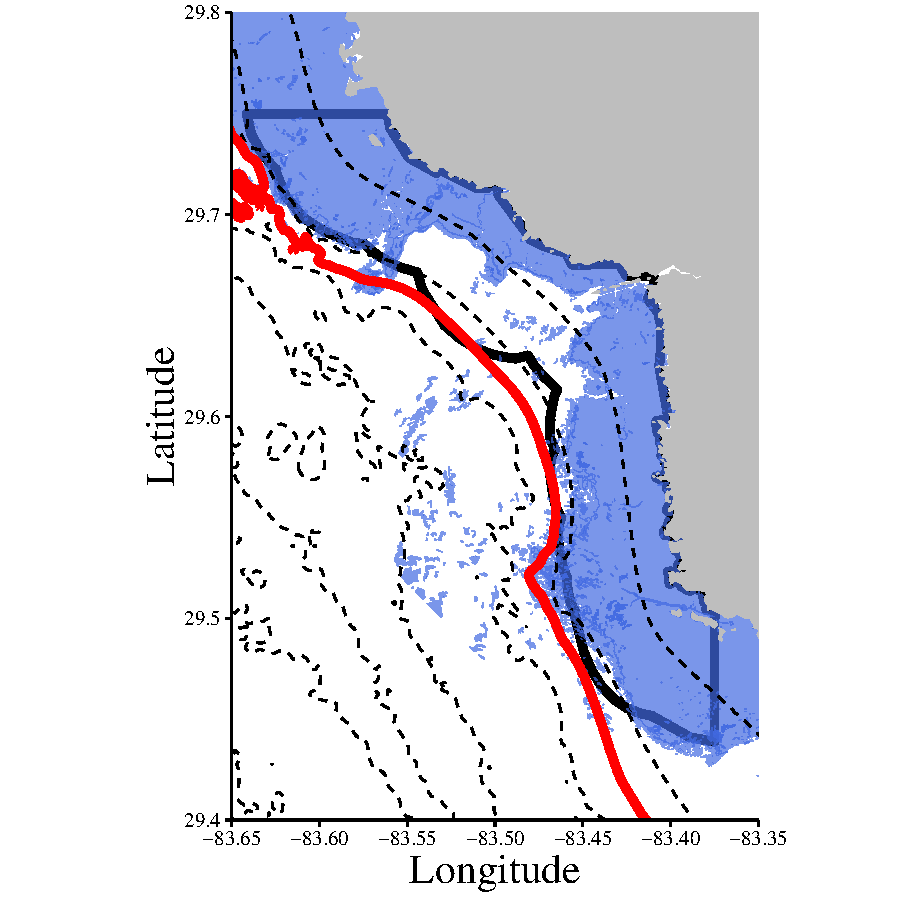
\includegraphics[width=0.5\textwidth,page=1]{figs/buff_ex.pdf}
\label{fig:buff_ex1}
}
\subfloat[][Grid of locations and sample areas for estimates]{
\includegraphics[width=0.5\textwidth,page=2]{figs/buff_ex.pdf}
\label{fig:buff_ex2}
}

\subfloat[][Sampled seagrass data for a test point]{
\includegraphics[width=0.5\textwidth,page=3]{figs/buff_ex.pdf}
\label{fig:buff_ex3}
}
\subfloat{
\includegraphics[width=0.5\textwidth,page=4]{figs/buff_ex.pdf}
}
\caption{Examples of data and grid locations for estimating seagrass depth of colonization for a region of the Big Bend, Florida.  \Cref{fig:buff_ex1} shows the seagrass coverage and depth contours at 2 meter intervals, including the whole segment estimate for depth of colonization. \cref{fig:buff_ex2} shows a grid of sampling locations with sampling radii for estimating \ac{doc} and seagrass depth points derived from bathymetry and seagrass coverage layers.  \cref{fig:buff_ex3} shows an example of sampled seagrass depth points for a test location.  Estimates in \cref{fig:est_ex} were obtained from the test location in \cref{fig:buff_ex3}.}
\label{fig:buff_ex}
\end{figure}

% example of depth of col ests for wbid - big bend 820
\begin{figure}
\centerline{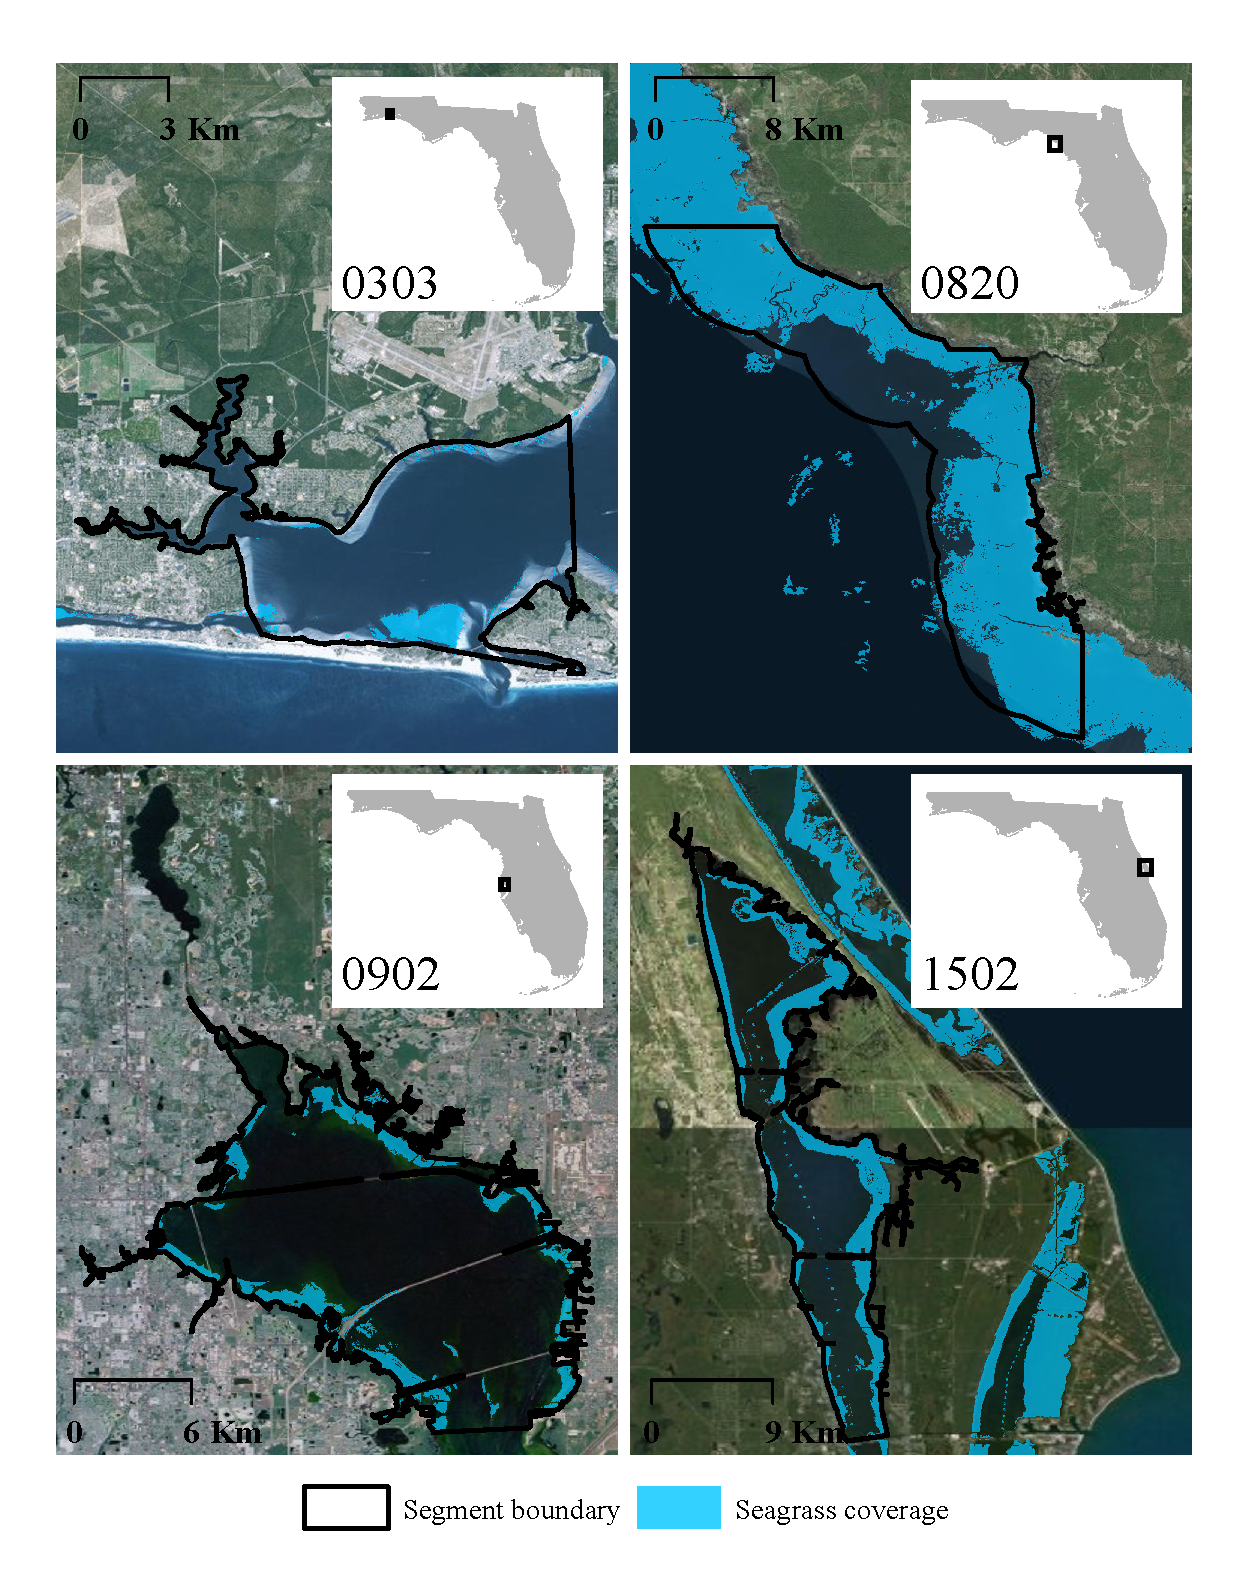
\includegraphics[width = \textwidth]{figs/seg_all.pdf}}
\caption{Locations and seagrass coverage of estuary segments used to evaluate \acl{doc} estimates.  Seagrass coverage layers are from 2006 (BB: Big Bend), 2010 (OTB: Old Tampa Bay), 2009 (UIRL: Upper Indian R. Lagoon), and 2007 (WCB: Western Choctawhatchee Bay).}
\label{fig:seg_all}
\end{figure}

% example of estimating seagrass depth of colonization


% example of depth of col ests for wbid - big bend 820
\begin{figure}
\centering
\subfloat[][Proportion of points with seagrass by depth]{
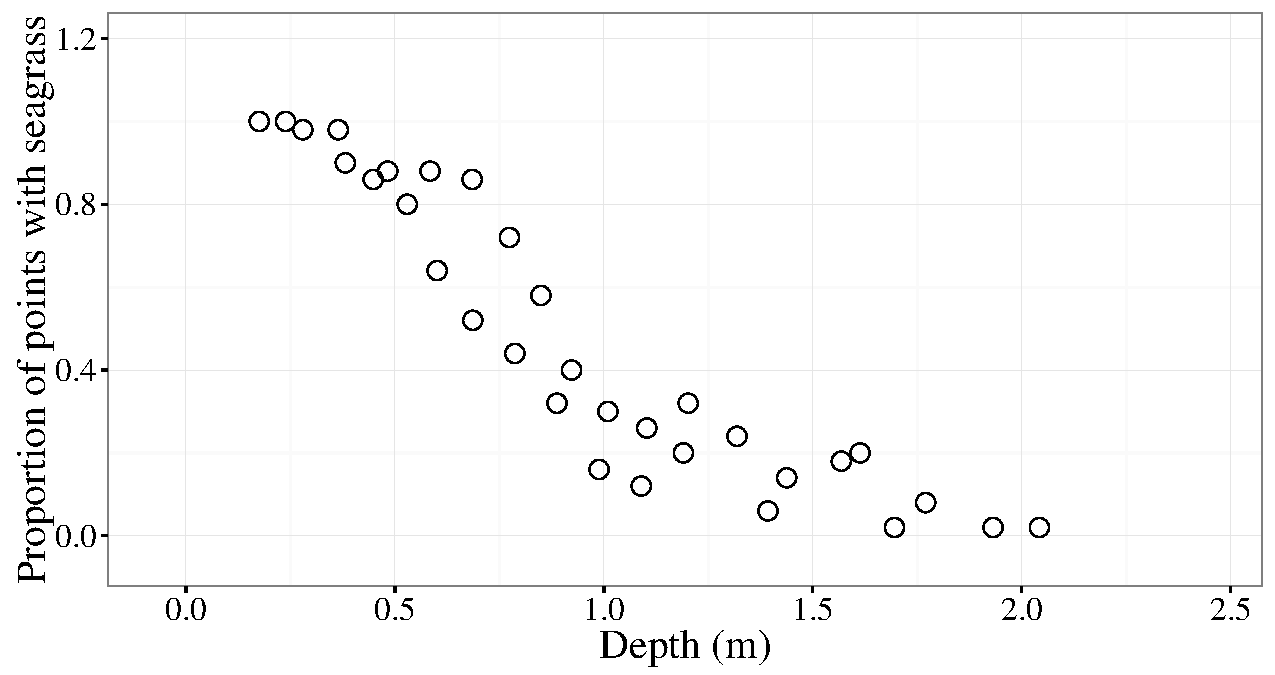
\includegraphics[page=1,width=0.5\textwidth]{figs/est_ex.pdf}
\label{fig:est_ex1}
}

\subfloat[][Logistic growth curve fit through points]{
\includegraphics[page=2,width=0.5\textwidth]{figs/est_ex.pdf}
\label{fig:est_ex2}
}

\subfloat[][Depth estimates]{
\includegraphics[page=3,width=0.5\textwidth]{figs/est_ex.pdf}
\label{fig:est_ex3}
}
\caption{Methods for estimating seagrass depth of colonization using sampled seagrass depth points around a single location. \Cref{fig:est_ex1} is the proportion of points with seagrass by depth using depth points within the buffer of the test point in \cref{fig:buff_ex}.  \Cref{fig:est_ex2} adds a decreasing logistic growth curve fit through the points.  \Cref{fig:est_ex3} shows three depth estimates based on a linear curve fit through the inflection point of logistic growth curve.}
\label{fig:est_ex}
\end{figure}

% grid examples for each segment

\begin{figure}
\centering
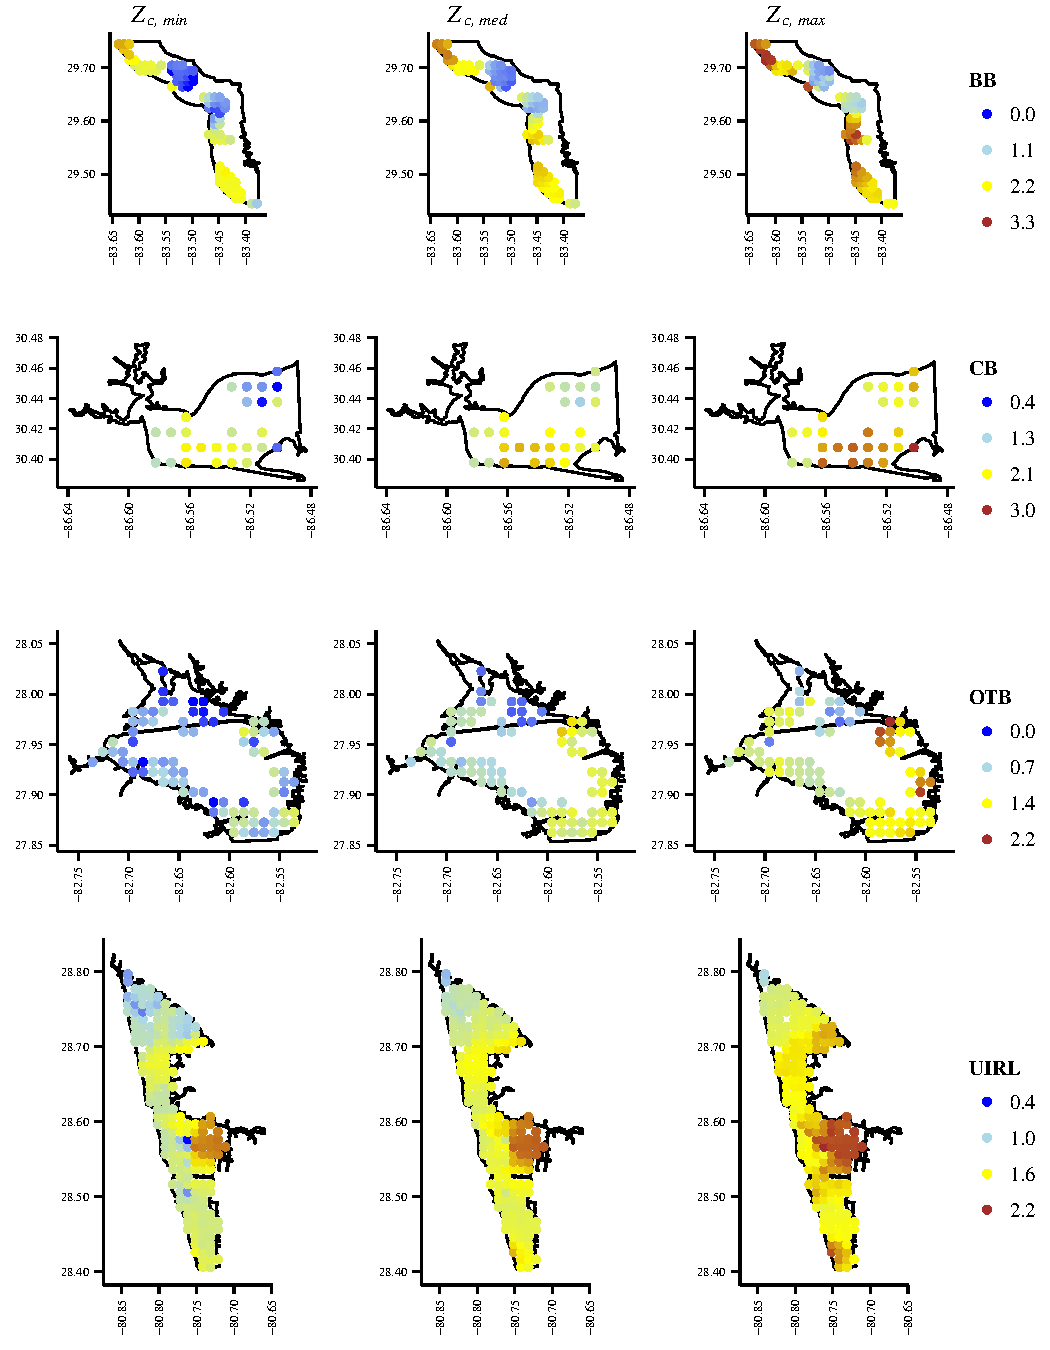
\includegraphics[width = 0.95\textwidth]{figs/all_ests.pdf}
\caption{Spatially-resolved estimates of seagrass depth limits (m) for four coastal segments of Florida. Maximum depth of colonization ($Z_{c,\,max}$) estimates are on the left and correspondings widths of the 95\% confidence intervals are on the right.  Estimates are assigned to grid locations for each segment, where grid spacing was fixed at 0.02 decimal degrees.  Radii for sampling seagrass bathymetric data around each grid location were fixed at 0.06 decimal degrees. From top to bottom: Big Bend, Old Tampa Bay, Upper Indian R. Lagoon, Western Choctawhatchee Bay.}
\label{fig:all_ests}
\end{figure}

% satellite estimates of water clarity for Tampa Bay

\begin{figure}
\centering
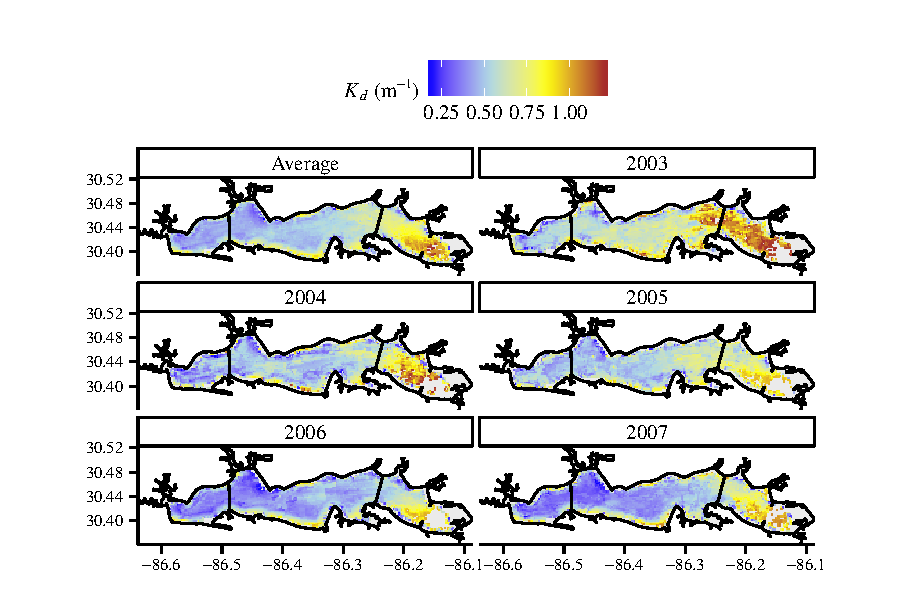
\includegraphics[width = \textwidth]{figs/kd_choc.pdf}
\caption{Satellite estimated light attenuation for Choctawhatchee Bay based on empirical relationships between \textit{in situ} secchi observations and surface reflectance.  Each facet is an annual average of light attenuation for available years of satellite data up to the year of seagrass coverage used to estimate depth of colonization.  The first facet is an average of all years.  See \cref{fig:light_choc} for segment identification.}
\label{fig:kd_choc}
\end{figure}

% satellite estimates of water clarity for Tampa Bay

\begin{figure}
\centering
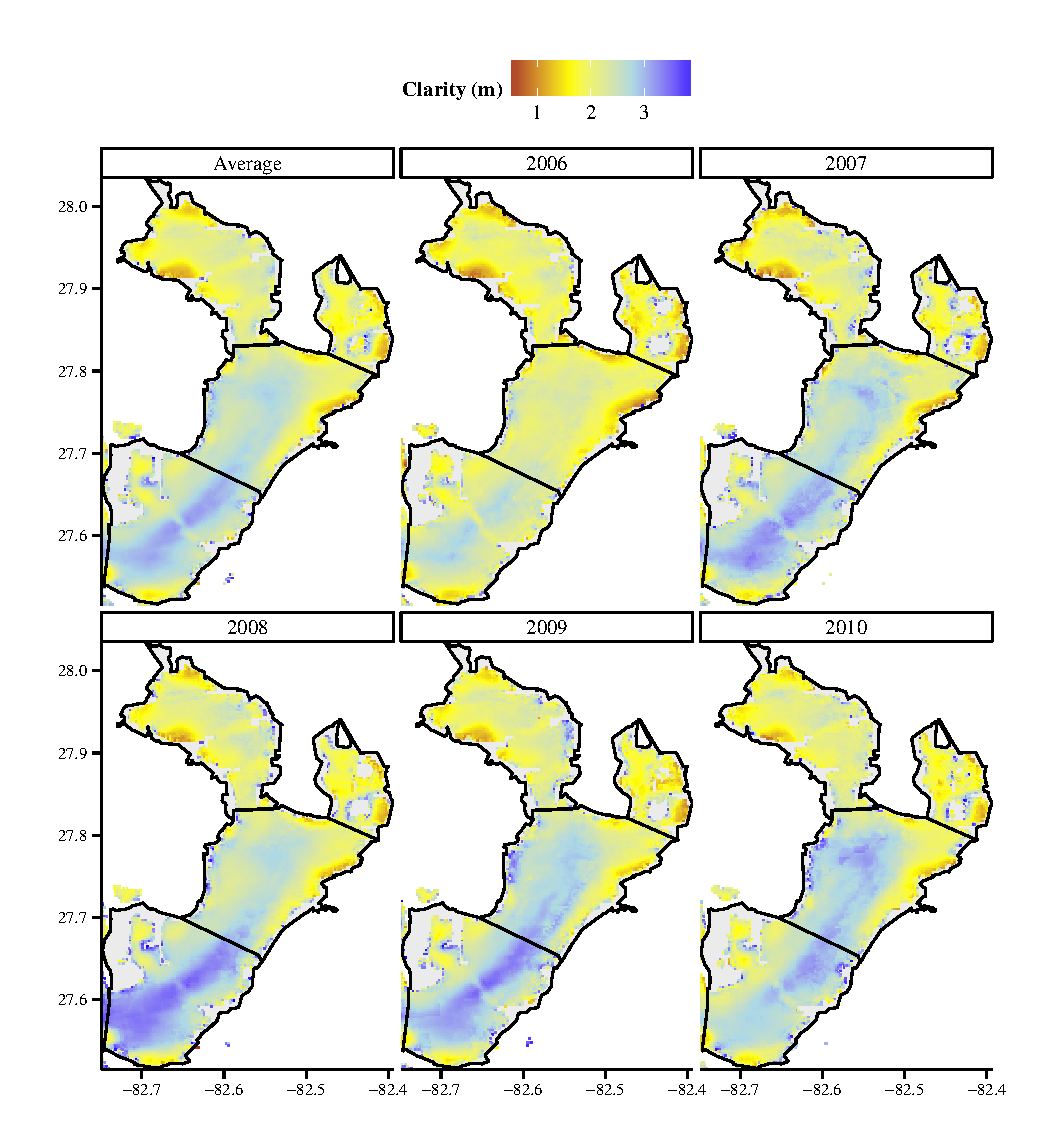
\includegraphics[width = \textwidth]{figs/clarity_tb.pdf}
\caption{Satellite estimated water clarity for Tampa Bay based on empirical relationships between \textit{in situ} secchi observations and surface reflectance.  Each facet is an annual average of water clarity for available years of satellite data. The first facet is an average of all years.  See \cref{fig:light_tb} for segment identification.}
\label{fig:clarity_tb}
\end{figure}

% estimated light requirements for Choctawhatchee Bay

\begin{figure}
\centering
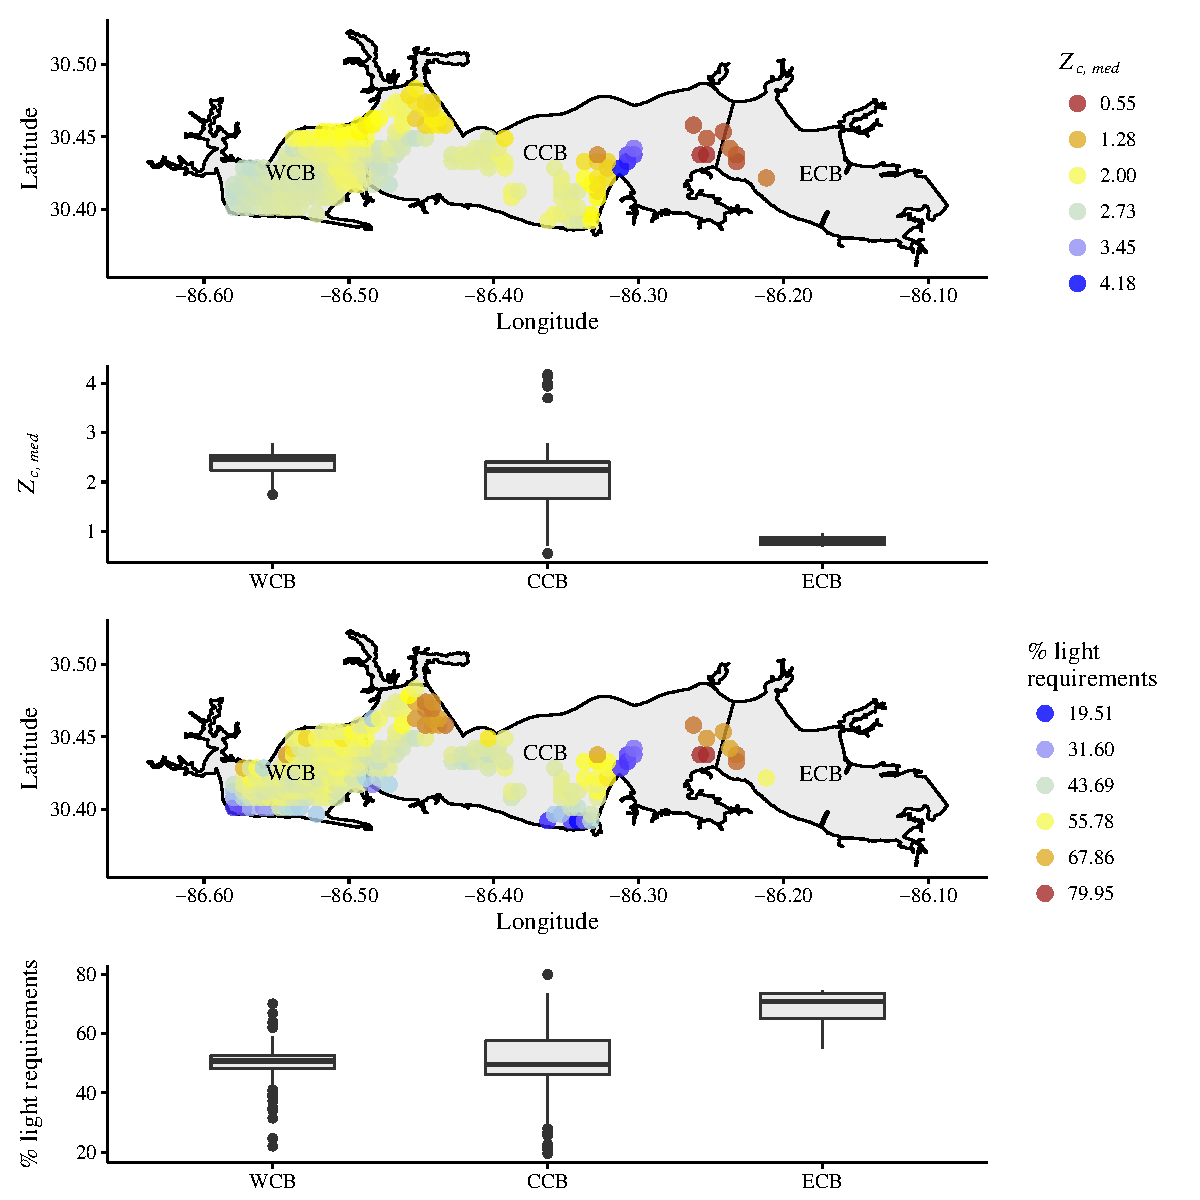
\includegraphics[width = 0.95\textwidth]{figs/light_choc.pdf}
\caption{Estimated maximum depths of seagrass colonization and light requirements for multiple locations in Choctawhatchee Bay, Florida. Locations are those where water clarity estimates were available from satellite observations and seagrass depth of colonization was estimable using a radius of 0.1 decimal degrees.  Estimates are also summarized by bay segment as boxplots where the dimensions are the 25\textsuperscript{th} percentile, median, and 75\textsuperscript{th} percentile.  Whiskers extend beyond the boxes as 1.5 multiplied by the interquartile range. CCB: Central Choctawhatchee Bay, ECB: East Choctawhatchee Bay, WCB: West Choctawhatchee Bay.}
\label{fig:light_choc}
\end{figure}

% estimated light requirements for Tampa Bay

\begin{figure}
\centering
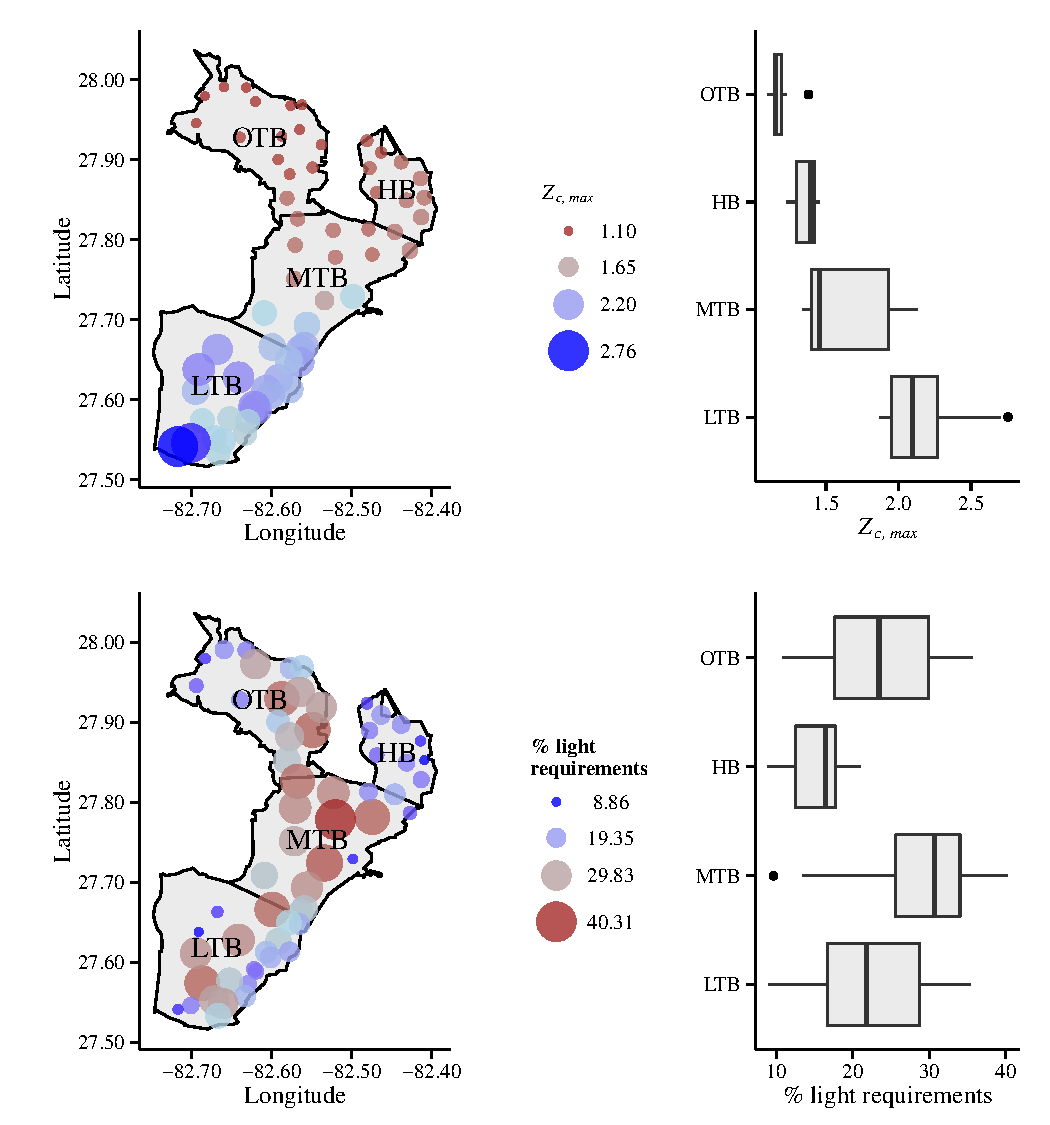
\includegraphics[width = 0.95\textwidth]{figs/light_tb.pdf}
\caption{Estimated maximum depths of seagrass colonization and light requirements for multiple locations in Tampa Bay, Florida. Locations are those where water clarity estimates were available from satellite observations and seagrass depth of colonization was estimable using a radius of 0.1 decimal degrees.  Estimates are also summarized by bay segment as boxplots where the dimensions are the 25\textsuperscript{th} percentile, median, and 75\textsuperscript{th} percentile.  Whiskers extend beyond the boxes as 1.5 multiplied by the interquartile range. HB: Hillsborough Bay, LTB: Lower Tampa Bay, MTB: Middle Tampa Bay, OTB: Old Tampa Bay.}
\label{fig:light_tb}
\end{figure}

% estimated light requirements for Indian River Lagoon

\begin{figure}
\centering
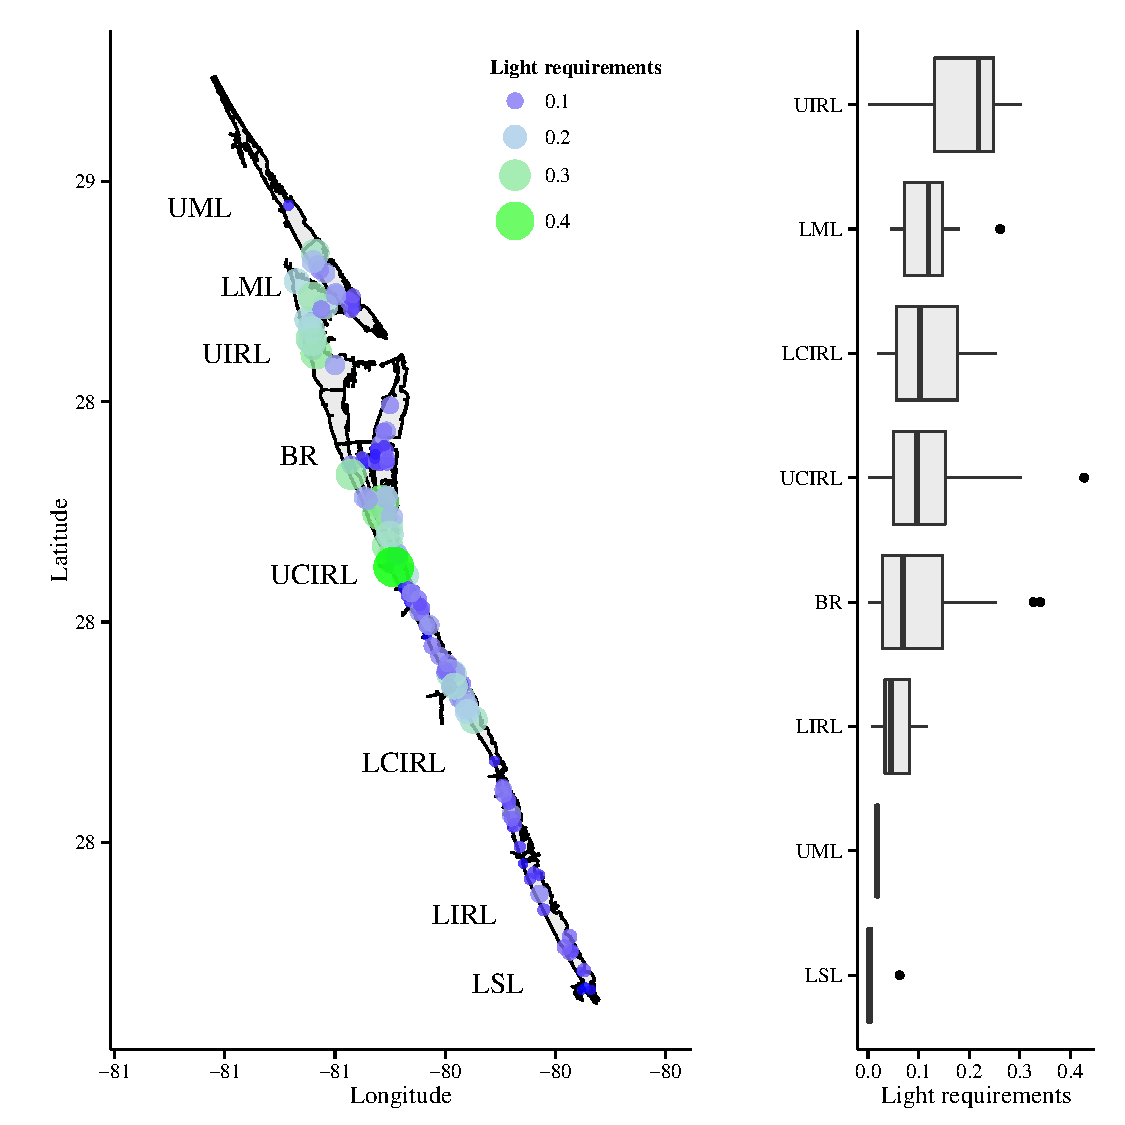
\includegraphics[width = 0.8\textwidth]{figs/light_irl.pdf}
\caption{Estimated maximum depths of seagrass colonization and light requirements for multiple locations in Indian River Lagoon, Florida.  Map locations are georeferenced observations of water clarity in the Florida \acl{IWR} database, update 40.  Estimates are also summarized by bay segment as boxplots as in \cref{fig:light_tb}. Light requirements are based on averaged secchi values within ten years of the seagrass coverage data and estimated maximum depth of colonization using a radius of 0.02 decimal degrees for each secchi location to sample seagrass depth points. BR: Banana R., LCIRL: Lower Central Indian R. Lagoon, LIRL: Lower Indian R. Lagoon, LML: Lower Mosquito Lagoon, LSL: Lower St. Lucie, UCIRL: Upper Central Indian R. Lagoon, UIRL: Upper Indian R. Lagoon, UML: Upper Mosquito Lagoon.}
\label{fig:light_irl}
\end{figure}

\end{document}
